\documentclass[border={1cm 1cm 1cm 1cm}]{standalone}

\usepackage{amssymb}
\usepackage{amsmath}	%for \frac
\usepackage{tikz}

%Various tempered scales and their relationship to Pythagorean ratios
%Wishart, Trevor. (1996). On Sonic Art. Amsterdam: Harwood Academic Publishers, p. 74 (fig. 4.2)

\begin{document}
	
	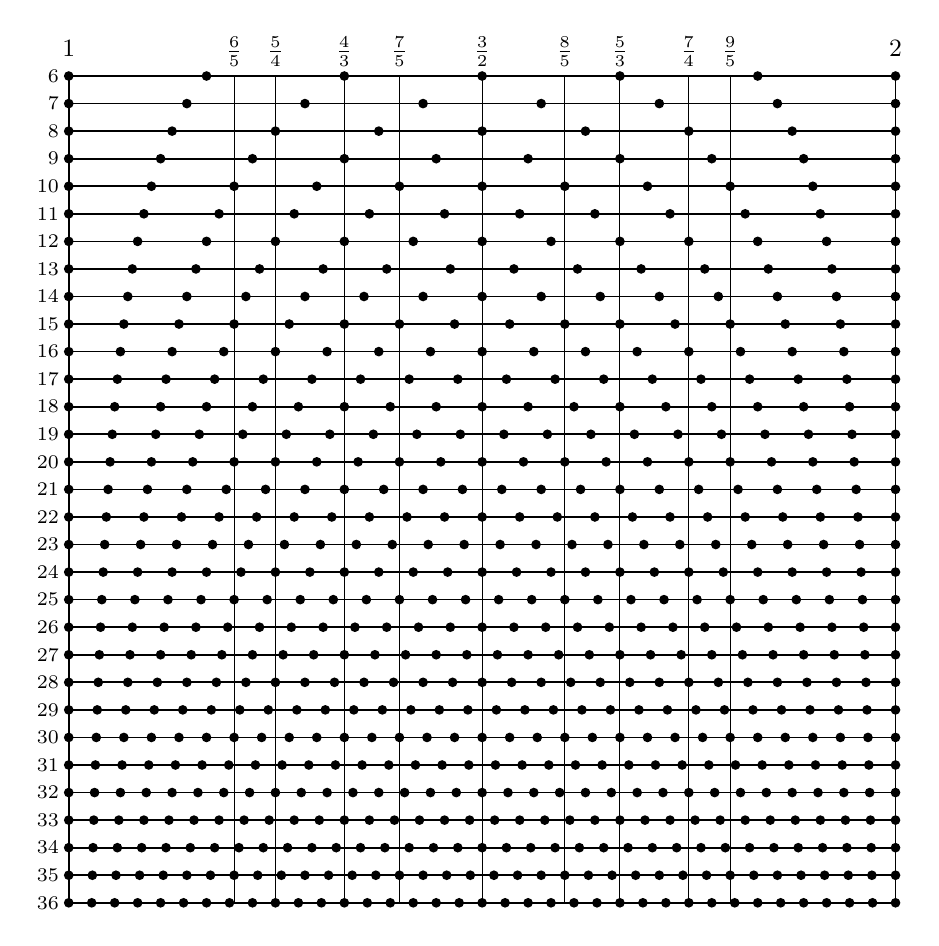
\begin{tikzpicture}
	%VERTICAL LINES
	\draw[semithick] (0,0)--(0,10.5);			\node at (0,10.85) {\small 1};
	\draw[semithick] (10.5,0)--(10.5,10.5);		\node at (10.5,10.85) {\small 2};

	%HORIZONTAL LINES
	\foreach \n in {6,...,36}{
		\draw[semithick] (0,10.5+6*10.5/30-\n*10.5/30)--(10.5,10.5+6*10.5/30-\n*10.5/30); %lines
		\node[align=left,left] at (0,10.5+6*10.5/30-\n*10.5/30) {\scriptsize \n}; %labels
		\foreach \x in {0,...,\n}{
		\fill (\x*10.5/\n,10.5+6*10.5/30-\n*10.5/30) circle (1.75pt);	%dots
		}	%end inner foreach
	}	%end outer foreach
	
	%PYTHAGOREAN RATIOS
	\foreach \n/\d in {6/5,5/4,4/3,7/5,3/2,8/5,5/3,7/4,9/5}{
		\draw ({(\n/\d-\d/\d)*10.5},10.5)--({(\n/\d-\d/\d)*10.5},0); %lines
		\node[align=center,above] at ({(\n/\d-\d/\d)*10.5},10.5) {\small $\frac{\n}{\d}$}; %labels
	}
	\end{tikzpicture}
	
\end{document}